\documentclass[]{exam}
\usepackage{epic,array,ecltree,url,calrsfs}
\usepackage[nointegrals]{wasysym}

%These tell TeX which packages to use.
\usepackage{array,epsfig}
\usepackage{amsmath}
\usepackage{amsfonts}
\usepackage{amssymb}
\usepackage{amsxtra}
\usepackage{amsthm}
\usepackage{mlextra} % must come after ams packages
\usepackage{mathrsfs}
\usepackage[dvipsnames]{xcolor}
\usepackage{array}
\usepackage{graphicx}
\graphicspath{ {../art/} }
\usepackage{bm}
\usepackage{tikz}
\usepackage{multicol}
\usepackage{enumitem}

\newcommand{\twonode}{%
  \begingroup\normalfont
  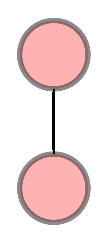
\includegraphics[height=\fontcharht\font`\b]{2nodetree.eps}%
  \endgroup
}


\title{Lab 4: Proving Properties of Mutually Recursive Systems}
\author{Foundations of Computer Science}
\date{\today}
%\pagestyle{empty} 
%\footer{}{\thepage}{}

\unframedsolutions
\SolutionEmphasis{\itshape\small}
\SolutionEmphasis{\color{NavyBlue}}

\begin{document}

\maketitle

\setlength{\columnseprule}{1pt}
\section*{Post System Practice}
\begin{questions}
\question Write a Post system that defines the negative integers.
\begin{solution}
\begin{tabbing}
{\bf R2}XX \=  \kill
{\bf B} \>
        \(\begin{array}[t]{l}
        -1 \in N
        \end{array}\) \\[2ex]
{\bf R} \>
        \(\begin{array}[t]{l}
        x \in N \\
        \hline
        x-1 \in N
        \end{array}\)
\end{tabbing}
\end{solution}
\question Write a Post system that defines even natural numbers greater than $6$.
\begin{solution}
\begin{tabbing}
{\bf R2}XX \=  \kill
{\bf B} \>
        \(\begin{array}[t]{l}
        8 \in N
        \end{array}\) \\[2ex]
{\bf R} \>
        \(\begin{array}[t]{l}
        x \in N \\
        \hline
        x+2 \in N
        \end{array}\)
\end{tabbing}
\end{solution}
\question Consider the following Post systems:
\begin{multicols}{2}
\begin{tabbing}
{\bf R2}XX \=  \kill
{\bf B} \>
        \(\begin{array}[t]{l}
        a \in S
        \end{array}\) \\[2ex]
{\bf R} \>
        \(\begin{array}[t]{l}
        x \in S \;\;\;y \in S \\
        \hline
        xy \in S
        \end{array}\)
\end{tabbing}

\begin{tabbing}
{\bf R2}XX \=  \kill
{\bf B} \>
        \(\begin{array}[t]{l}
        a \in T
        \end{array}\) \\[2ex]
{\bf R} \>
        \(\begin{array}[t]{l}
        x \in T \\
        \hline
        xx \in T
        \end{array}\)
\end{tabbing}

\end{multicols}
\begin{parts}
\part\label{ques:defSandT} Write definitions for $S$ and $T$ using set comprehension notation.
\begin{solution}
~\\
$S = \{a^k | k \in \Z^+\}$ (Note: $\Z^+$ refers to the positive integers.)\\
$T = \{a^{2^k} | k \in \N_0\}$ (Note: $\N_0$ refers to the non-negative
    integers.)\\
As discussed in class, there are many other ways of defining these sets. For
example, you could first define $\Sigma = \{a\}$, and then $S = \Sigma^+$.

\end{solution}
\part Is $S$ equal to $T$?
\begin{solution}
No.
\end{solution}
\part Bonus practice: Prove $T \subseteq S$.
\begin{solution}
\begin{proof}
We prove by weak induction on derivation height of
$T$ that all elements of $T$ can be derived in the system that defines $S$.\\
$S(0)$: If derivation height of an element $x \in T$ is $0$, then $x$ must have 
been produced using rule $B$. The only such element is $x = a$. However, $a$ can 
be derived immediately from the axiom of $S$, so $a \in S$.\\
$S(n)$: We assume that if the derivation height of an element in $T$ is $n$,
for $n \geq 0$, then $n \in S$.\\
$S(n+1)$: Let $y \in T$ such that the derivation height of $y$ is $n+1$. Then
$y$ is produced by rule $R$, and therefore has the form $y = x'x'$, where $x' \in T$
and $x'$ has derivation height $n$. By the inductive hypothesis, $x' \in S$. Using
rule $R$ in the Post system for $S$ and choosing $x'$ for both the $x$ and $y$ 
inputs, we have $xy = x'x' \in S$, which completes the proof.
\end{proof}

Further notes: Assuming you have correctly translated the Post systems into
set comprehensions, it is also possible to prove $S \subseteq T$ by showing
an arbitrary element described by the comprehension for $T$ is also described
by the comprehension given for $S$. The argument will depend on how the sets 
have been described. Here is a proof using this method with the set comprehension 
definitions given for $S$ and 
$T$ in the solution to question (\ref{ques:defSandT}) above:
\begin{proof}
If $x \in T$ then $x = a^{2^k}$. Let $k' = 2^k$. Then $x = 2^{k'}$ and 
$k' \in \Z^+$ (since $k \in \N_0$), so $x \in T$.
\end{proof}
Strictly speaking, one would have to first prove that the set comprehensions 
given are a correct representation of the sets defined by the Post
systems---i.e., that the solution given to question (\ref{ques:defSandT}) 
is in fact correct.  
\end{solution}
\end{parts}

\question Consider the following Post system:

\begin{tabbing}
{\bf R2}XX \=  \kill
{\bf B} \>
        \(\begin{array}[t]{l}
        1 \in N
        \end{array}\) \\[2ex]
{\bf R1} \>
        \(\begin{array}[t]{l}
        x \in N \\
        \hline
        x\times x \in S
        \end{array}\)\\[2ex]
{\bf R2} \>
        \(\begin{array}[t]{l}
        x \in S \;\;\; y \in N \\
        \hline
        x+y \in N
        \end{array}\)
\end{tabbing}
\begin{parts}
\part List $5$ elements of $S$ and $5$ elements of $N$.
\begin{solution}
(Note the altered definition creates a simpler system than the original
 version.)\\
$S = \{1,4,9,16,25...\}$\\
$N = \{1,2,3,4,5...\}$
\end{solution}

\part Use set comprehension notation to write definitions of $S$ and $N$. 
\begin{solution}
~\\
$S = \{n^2| n \in \Z^+\}$\\
$N = \Z^+$
\end{solution}
\end{parts}

\newpage
\uplevel{\section*{Trees}
Answer the questions below referring to the following definitions:
\begin{itemize}
\item A ``leaf'' node is a node with no children.
\item An ``internal'' node is a node that is not a leaf.
\item A full binary tree is a tree in which every internal node
      has exactly two children.
\item An extended binary tree is a tree in which every internal
      node has one or two children.
\end{itemize}}
\hrule
%This week: strong induction vs. weak induction.
%Mutual recursive definition and mutual induction.

\question Write a Post System for full binary trees.
\begin{solution}
\begin{tabbing}
{\bf R2}XX \=  \kill
{\bf B} \>
        \(\begin{array}[t]{l}
        \id{nil}\in\id{RTL}
        \end{array}\) \\[2ex]
{\bf R1} \>
        \(\begin{array}[t]{l}
        t\in\id{RT}\;\;\;u\in\id{RT} \\
        \hline
        \id{cons}(t,\id{cons}(u,nil))\in\id{RTL}
        \end{array}\) \\[2ex]
{\bf R2} \>
        \(\begin{array}[t]{l}
        l\in\id{RTL} \\
        \hline
        \id{node}(l)\in\id{RT}
        \end{array}\)
\end{tabbing}

\end{solution}
\question Write a Post System for extended binary trees.
\begin{solution}
\begin{tabbing}
{\bf R2}XX \=  \kill
{\bf B} \>
        \(\begin{array}[t]{l}
        \id{nil}\in\id{RTL}
        \end{array}\) \\[2ex]
{\bf R1} \>
        \(\begin{array}[t]{l}
        t\in\id{RT}\;\;\;u\in\id{RT} \\
        \hline
        \id{cons}(t,\id{cons}(u,nil))\in\id{RTL}
        \end{array}\) \\[2ex]
{\bf R2} \>
        \(\begin{array}[t]{l}
        t\in\id{RT} \\
        \hline
        \id{cons}(t,nil)\in\id{RTL}
        \end{array}\) \\[2ex]
{\bf R3} \>
        \(\begin{array}[t]{l}
        l\in\id{RTL} \\
        \hline
        \id{node}(l)\in\id{RT}
        \end{array}\)

\end{tabbing}

\end{solution}

% Question below omitted because:
% It needs work, is too challenging, and there is already too much material.
%\question Let $L$ be the number of leaf nodes and $I$ be the number
%          of internal nodes. Suppose you are asked to prove that for all 
%          full binary trees, $L = I + 1$.
%\begin{parts}
%\part What induction rule should you use? 
%\begin{solution}
%Strong mutual induction with multiple base cases.  
%\end{solution}
%\part What variable will you perform induction over? 
%\begin{solution}
%Derivation height.
%\end{solution}
%\part Set up the proof: write the base case, inductive hypothesis and inductive step.
%\begin{solution}
%~\\{\bf Base Cases:}\\
%$S_1(0), S_1(1), S_1(2)$: If the derivation of $l\in \id{RTL}$ has height $0$,
%  $1$ or $2$, then $L = I + |l|$.
%
%$S_2(0), S_2(1), S_2(2)$: If the derivation of $t\in \id{RT}$ has height $0$,
%  $1$ or $2$, then $L = I + 1$.
%
%{ \bf Inductive Hypothesis:}\\
%$S_1(k)$: If the derivation of $l\in \id{RTL}$ has height $k$ where $2 \leq k
%\leq n$ and $n \geq 0$, then $L = I + |l|$.
%
%$S_2(k)$: If the derivation of $t\in \id{RT}$ has height $k$ where $2 \leq k
%\leq n$ and $n \geq 0$, then $L = I + 1$.
%
%{\bf Inductive Step:}\\
%$S_1(n+1)$: Assuming the inductive hypothesis, we must show if the derivation of $l\in \id{RTL}$ 
%            has height $n+1$ then $L = I + |l|$.
%
%$S_2(n+1)$: Assuming the inductive hypothesis, we must show if the derivation of $t\in \id{RT}$ 
%            has height $n+ 1$ then $L = I + 1$.
%
%
%\end{solution}
%\part Prove the base case.
%\begin{solution}
%%omitted
%~\\
%$S_1(0)$: If the derivation of $l\in \id{RTL}$ has height $0$, it was
%produced by rule $B$. Therefore, it is the empty list, so $L = I = |l| = 0$,
%and $ 0 = 0 + 0$, so the formula holds.
%
%$S_2(0)$: There is no $t\in \id{RT}$ with a derivation height of $0$. Therefore
%this statement is vacuously true. 
%
%$S_1(1)$: If the derivation of $l\in \id{RTL}$ has height $1$, then it was
%produced by rule $R1$. However, this implies that it has the form $cons(t,u)$
%where the derivation height of $t,u \in RT$ is $0$. Since no elements of $RT$
%have a derivation height of $0$, this is false, so the implication is vacuously
%true.
%
%$S_2(1)$: If $t\in \id{RT}$ has a derivation height of $1$, it has the form
%$node(l)$ where $l \in RTL$ has a derivation height of $0$. Therefore
%$l$ was produced by rule $B$, so $l$ is the empty list, and the tree $t$ is a
%single root. The root $t$ has no children, so it is a leaf, and $t$ has no
%internal nodes. Therefore subsituting into $L = I + 1$ gives $1 = 0 + 1$,
%and the formula holds.
%
%$S_1(2)$: If the derivation of $l\in \id{RTL}$ has height $2$, then it was
%produced by rule $R1$. This implies that it has the form $cons(t,u)$
%where the derivation height of $t,u \in RT$ is $1$. Therefore both $t$ and $u$
%have the form $node(l')$ where $l'$ has a derivation height of $0$, and is
%therefore the empty list. Consequently, both $t$
%and $u$ are single node trees, and both have a single leaf and no internal
%nodes. It follows that $l$ has $2$ leaf nodes and $0$ internal nodes, so
%substituting for the formula $L = I + |l|$ gives $2 = 0 + 2$, which is correct.
%
%$S_2(2)$: If $t\in \id{RT}$ has a derivation height of $2$, it has the form
%$node(l)$ where $l \in RTL$ has a derivation height of $1$. However, this
%implies $l$ has the form $cons(t,u)$, where $t$ and $u$ have a derivation
%height of $0$, which is impossible, since there is no axiom that produces
%elements of $RT$. Therefore the premise is false, and the implication
%is vacuously true.
%%
%\end{solution}
%\part Prove the inductive step.
%\begin{solution}
%%omitted
%\begin{proof}
%$S_1(n+1)$: If the derivation of $l'\in \id{RTL}$ has height $n+1$ then it was
%produced by rule $R1$ so it has the form $ l' = cons(t,u)$, where $t$ and $u$ are
%in $RT$ and have derivation height $k$, where $2 \geq k \geq n$. Let $L$ be the
%number of leaf nodes in $l'$, $L_t$ be the number of leaf nodes in $t$ and $L_u$ 
%be the number of leaf nodes in $u$. Similarly, let $I, I_t,I_u$ represent the
%number of internal nodes in $l',t,u$, respectively. Clearly, $L' = L_t + L_u$
%and $I = I_t + I_u$. Moreover, by the inductive hypothesis $S_2$, we have 
%$L_t = I_t + 1$ and $L_u = I_u + 1$. Thus, $L =  L_t + L_u = I_t + 1 + I_u + 1 =
%I_t + I_u + |l'| = I + |l'|$. This proves $S_1(k) \land S_2(k) \implies S_1(n+1)$
%where $2 \leq k \leq n$.
%
%$S_2(n+1)$: All elements of $\id{RT}$ are produced by $R2$ so if $t' \in RT$
%and $t'$ has a derivation height of $n+ 1$ then it has the form $node(l)$, where 
%$l \in RTL$ and $l$ has a derivation height of $n$. Since $2 \leq k \leq n$, 
%$n$ is a possible value of $k$ and the inductive hypothesis applies.  Let $L, I$ 
%be the number of leaf nodes and internal nodes in $t'$, respectively, and 
%let $L_l,I_l$ be the number of leaf nodes and internal nodes in $l$. Since the 
%derivation height of $l$ is at least $2$ it must have been produced by
%rule $R1$. Therefore $|l| = 2$ and $l = cons(t,u)$, where $t$ and $u$ have
%derivation heights of at least $1$ (and thus contain at least one node).
%It follows that $L = L_l$, since the process of forming a tree with $node$ 
%does not add any more leaves, and $I = I_l + 1$, since forming a tree from 
%the trees in $l$ produces one extra internal node (the new root). By the 
%inductive hypothesis, we have that $L_l = I_l + |l|$, so by substitution 
%$L = I_l + |l|$. Moreover, because $|l| = 2$, $L = I_l + |l| = I_l + 1 + 1 = I +
%1$. This proves $S_1(k) \land S_2(k) \implies S_2(n+1)$ where $2 \leq k \leq n$.
%\end{proof}
%\end{solution}
%\end{parts}
\uplevel{\section*{Simple Automata}}
\question The diagram below shows a slightly modified version of the simple
switch discussed in class. \\
\begin{figure}[h]
\centering
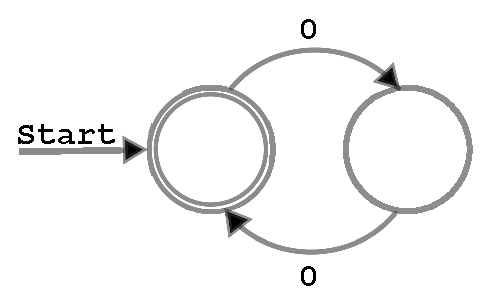
\includegraphics[width=2.5in, height=.75in,keepaspectratio=true]{evenzeroautomata.eps}
\label{2sp}
\end{figure}

There are two changes:
\begin{itemize}
\item Instead of a button labeled ``Push,'' this machine has a single button
labeled ``0''. Pressing the button represents sending the character ``0''
to the machine, which results in a state transition, just as it did when labeled
``Push'' in the previous version.
\item The double circle shown for the start state indicates that this is an
``accepting'' state. If the machine is in an accepting state after processing
all its input, it has accepted the input. If it ends in any other state, it has
rejected the input.
\end{itemize}
For the following questions, let $L$ be the set of all strings accepted by this machine. 
We refer to this set as the language recognized by the machine.

\begin{parts}
\part What is the alphabet of $L$?
\begin{solution}
$\{0\}$
\end{solution}
\part\label{ques:defL} Define $L$ using set comprehension notation. 
\begin{solution}
$L = \{0^{2k} | k \in \N_0\}$
\end{solution}

\part\label{ques:completeness} What induction rule would you use to prove that 
all the strings contained in the set $L$ as you have defined it are accepted by 
the machine? What variable should you do induction over?
\begin{solution}
Weak induction on $k$ (see definition of $L$ given in (\ref{ques:defL})). Note that 
answers may vary---in particular, you could also use strong induction on the length 
of an even-length string of $0$s.
\end{solution}
\part\label{ques:soundness} What induction rule would you use to prove that all the 
strings accepted by the machine are contained in the set $L$ as you have defined it? What
variable should you do induction over?
\begin{solution}
Mutual weak induction on input length.
\end{solution}
\part Which of the above proves soundness of the machine with respect to $L$, and 
which proves completeness? 
\begin{solution}
(\ref{ques:soundness}) proves soundness of the set of strings the machine accepts 
(i.e., it \emph{only} accepts strings of even length).
(\ref{ques:completeness}) proves completeness of the set of strings the machine
accepts (i.e., it accepts \emph{all} strings of even length).
\end{solution}
\part Sketch the proof of completeness.
\begin{solution}
Let $x$ be an even length string of $0$s. Then $x$ has the form $x = 0^{2k}$,
  where $k \in N_0$. We prove by weak induction on $k$ that the automaton
  accepts all strings of this form.\\
{\bf $S(0)$ (the base case):} the automaton accepts the string $x = 0^{2\cdot 0}$.\\ 
{\bf  $S(k)$ (the inductive hypothesis):} the automaton accepts
  strings of the form $0^{2k}$, for $k \geq 0$.\\
{\bf $S(k + 1)$ (the inductive step):} We must show that the inductive hypothesis
  implies that the automaton accepts strings of the form $0^{2(k+1)}$.
\end{solution}
 
\part Prove the base case.
\begin{solution}
$S(0)$: $x = 2^0 = \epsilon$. The automata starts in an accepting state. Since
the input is the empty string, no transitions are made, so the automaton ends
in an accepting state.
\end{solution}
\part Prove the inductive step.
\begin{solution}
We must show that the automaton accepts the string $y$ where $y = 0^{2(k+1)}$.
By definition of the concatenation operation, we can rewrite $y$ as $x00$,
where $x = 0^{2k}$. We know by the inductive hypothesis that the automaton 
accepts strings of the form $0^{2k}$, for $k \geq 0$, so it will be in an
accepting state after consuming the characters of $x$. Then, by the state
diagram, consuming the two remaining $0$ characters will cause the automaton
to transition first to the non-accepting state (on the first $0$) and then
back to the accepting state (on the second $0$). Since these are the only
possible transitions, the automaton must be in an accepting state after
consuming the entire string $y$. This proves the inductive step.
\end{solution}
\end{parts}
\end{questions}
\end{document}


